\documentclass[10pt]{article}

\usepackage[letterpaper,left=0.75in,right=0.75in,top=1in,bottom=1in]{geometry}

\usepackage[T1]{fontenc}
\usepackage[utf8]{inputenc}
\usepackage{lmodern}

\usepackage[activate={true,nocompatibility},final,tracking=true,kerning=true,spacing=true,factor=1100,stretch=10,shrink=10]{microtype}
\microtypecontext{spacing=nonfrench}
\usepackage{xspace}
\usepackage{amssymb,amsfonts,amsmath}
\usepackage{lipsum,xcolor}
\usepackage{graphicx}
\usepackage{float,caption,subcaption,wrapfig}
\usepackage{tcolorbox}
\usepackage{listings}
\usepackage{courier}
\usepackage[english]{babel}
\usepackage{textcomp}
\usepackage{enumitem}
\usepackage{csquotes}
\usepackage{siunitx}
\usepackage[makeroom]{cancel}
\sisetup{mode=text,
         group-separator={,},
         detect-all,
         binary-units,
         list-units = single,
         range-units = single,
         range-phrase = --,
         per-mode = symbol-or-fraction,
         list-final-separator = {, and }
}

\lstset{basicstyle=\ttfamily,
        breaklines=true,
        numbersep=-8pt,
        numberstyle=\small,
        numbers=right,
        frame = single, 
        showstringspaces=false,    
        keywordstyle=\color{blue}\bf,
        commentstyle=\color{darkgray},
        stringstyle=\color{purple}\bf,
  }

\DeclareSIUnit\atm{atm}
\DeclareSIUnit\bar{bar}

\headheight = 13.6pt
\usepackage{fancyhdr}
\pagestyle{fancy}

\lhead{PH 641 Sp2020}
\chead{Assignment 1}
\rhead{Due 11:59 pm, 17 March 2020}

\rfoot{Submitted by: Paige Lorson}
\tcbset{width=(\linewidth-2mm),before=,after=\hfill,colframe=black,colback=white,}
\newcommand{\volume}{{\ooalign{\hfil$V$\hfil\cr\kern0.08em--\hfil\cr}}}
\newenvironment{Solution}
    {\textbf{Solution:}
    
    \vspace{5mm}
    \begin{tcolorbox}
    }
    {
    \end{tcolorbox}
    \vspace{5mm}
    % \newpage
    }
\newcommand{\vol}{{\ooalign{\hfil$V$\hfil\cr\kern0.08em--\hfil\cr}}}
\renewcommand\labelitemi{$\cdot$}

\begin{document}

% \noindent\textbf{Note:} This survey serves to inform your instructor and to test the homework submission via gradescope. It will be graded like a regular homework set.

\begin{enumerate}

%%%%%%%%%%%%%%%%%%%%%%%%%%%%%%%%%%%%%%%%%%%%%%%

\item A fluid undergoes an adiabatic throttling process. Throttling means that the fluid is pressed through a porous plug, with initial (constant) pressure $p_{1}$ and final (constant) pressure $p_{2}$

\begin{enumerate}

\item Show that the enthalpy of the fluid is constant in this process. As a result of this process, the temperature changes (remember when you pump air in your bicycle tire, or when you let the air escape?). The amount of change is measured by the Joule-Thomson coefficient $\eta_{J T}$, defined by
$$
\eta_{J T}=\left.\frac{\partial T}{\partial p}\right|_{H}
$$

\begin{Solution}
In general for an open system,

\begin{align}
\dot{m}_{i n}\left(h_{i n}+\frac{1}{2} \vec{V}_{i n}^{2}+g z_{i n}\right)+\dot{Q}_{i n}+\dot{W}_{i n} 
=\dot{m}_{o u t}&\left(h_{o u t}+\frac{1}{2} \vec{V}_{o u t}^{2}+g z_{o u t}\right) \\
&+\dot{Q}_{o u t}+\dot{W}_{o u t}+\frac{d U}{d t}+\frac{d K E}{d t}+\frac{d P E}{d t}
\end{align}

For a throttling valve, we can assume steady flow, no change in elevation, negligible heat transfer, and no work in or out. 

\begin{align}
\dot{m}_{i n}\left(h_{i n}+\frac{1}{2} \vec{V}_{i n}^{2}+g \bcancel{z_{i n}}\right)+\bcancel{\dot{Q}_{i n}}+\bcancel{\dot{W}_{i n}}
=\dot{m}_{o u t}&\left(h_{o u t}+\frac{1}{2} \vec{V}_{o u t}^{2}+g \bcancel{z_{o u t}}\right) \\
&+\bcancel{\dot{Q}_{o u t}}+\bcancel{\dot{W}_{o u t}}+\bcancel{\frac{d U}{d t}}+\bcancel{\frac{d K E}{d t}}+\bcancel{\frac{d P E}{d t}}
\end{align}
\begin{equation}
    h_{i n}+\frac{1}{2} \vec{V}_{i n}^{2} = h_{o u t}+\frac{1}{2} \vec{V}_{o u t}^{2}
\end{equation}
In most cases, the change in velocity is rater small so the change in $KE$ can be neglected. This leaves us with
\begin{equation}
    \boxed{h_{in} = h_{out}}
\end{equation}
\end{Solution}

\item Show that
$$
\eta_{J T}=\frac{V}{C_{p}}(T \alpha-1)
$$

\begin{Solution}
\begin{align}
    \eta_{JT} &= \left.\frac{\partial T}{\partial p}\right|_H = - \left.\frac{\partial T}{\partial H}\right|_p \left.\frac{\partial H}{\partial p}\right|_T\\
    & = -\frac{1}{C_p} \left.\frac{\partial H}{\partial p}\right|_T
\end{align}
From $TdS$, 
\begin{equation}
    \left.\frac{\partial H}{\partial p}\right|_T = T \left.\frac{\partial S}{\partial p}\right|_T + V
\end{equation}
and from Maxwell's equations, 
\begin{equation}
    \left.\frac{\partial S}{\partial p}\right|_T = -V \alpha
\end{equation}
So,
\begin{equation}
    \boxed{ \eta_{J T}=\frac{V}{C_{p}}(T \alpha-1) }
\end{equation}
\end{Solution}

\item What is the value of $\eta_{J T}$ for an ideal gas?

\begin{Solution}
\begin{equation}
    \eta_{J T}=0
\end{equation}
\end{Solution}

\item What is the value of $\eta_{J T}$ for a van der Waals gas?
Remark: The temperature change of liquids and gases upon throttling is important for refrigeration and liquefaction of gases. A simpler effect is free expansion (discussed in class) and technical processes for the liquefaction of gases are the Linde cycle, Joule-Thompson effect plus heat exchanger, and Claude cycle, i.e a Linde cycle $+$ expansion engine. See for example Kittel and Kroemer, chapter 12.

\begin{Solution}
in the van der waal equation we can not solve for $V$ explicitly, so we need a different way to get$ \left.\frac{\partial T}{\partial p}\right|_{H}$. We can start with the $dH$ expression

\begin{equation}
    dH = \left.\frac{\partial H}{\partial T}\right|_{p}dT +\left.\frac{\partial H}{\partial p}\right|_{T}dp 
\end{equation}
recall $dH=0$ so, 
\begin{equation}
    \left.\frac{\partial H}{\partial T}\right|_{p}dT +\left.\frac{\partial H}{\partial p}\right|_{T}dp = 0
\end{equation}
\end{Solution}
% \newpage
    
\end{enumerate}

\newpage

%%%%%%%%%%%%%%%%%%%%%%%%%%%%%%%%%%%%%%%%%%%%%%%%%%%%%%%

\item \textbf{Van der Waals Gas} The van der Waals equation of state is given by
$$
\left(p+a \frac{N^{2}}{V^{2}}\right)(V-N b)=N R T
$$
where $a, b$ are positive constants and the volume $V$ is restricted to $V>N b$. It is a frequently used equation of state to study the liquid-gas phase transition. As such the van der Waals equation of state has regions of varying degrees of stability (stable, unstable, metastable).

\begin{enumerate}

\item Show that mechanical stability (i.e. compressibilities are positive) leads to the following condition for the unstable region of the van der Waals equation of state:
$$
n(1-n b)^{2} \geq \frac{R T}{2 a}
$$
where $n=N / V$
For temperatures $T$ above a critical temperature $T_{c}$ no instabilities occur for the van der Waals equation of state.

\begin{Solution}
\begin{equation}
\left.\frac{\partial p}{\partial V}\right|_{T, N}=-\frac{N R T}{V^{2}}\left(\frac{1}{(1-n b)^{2}}-2 a \frac{n}{R T}\right)< 0 
\end{equation}
\begin{equation}
\frac{N R T}{V^{2}}\left(\frac{1}{(1-n b)^{2}}-2 a \frac{n}{R T}\right)> 0 
\end{equation}
\begin{equation}
\frac{1}{(1-n b)^{2}}> 2 a \frac{n}{R T}
\end{equation}
\begin{equation}
n(1-n b)^{2} > \frac{R T}{2 a}
\end{equation}

\end{Solution}

\item Sketch in a $p-V$ diagram 3 isotherms of the van der Waals equation of state for $T_{1}>T_{c}, T_{c},$ and $T_{2}<T_{c} .$ Pay attention to slopes where they matter. Indicate in your p-V diagram the critical point $T_{c}\left(p_{c}, V_{c}\right)$ and different regions of stability and their boundaries (explain).

\begin{Solution}

\centering{
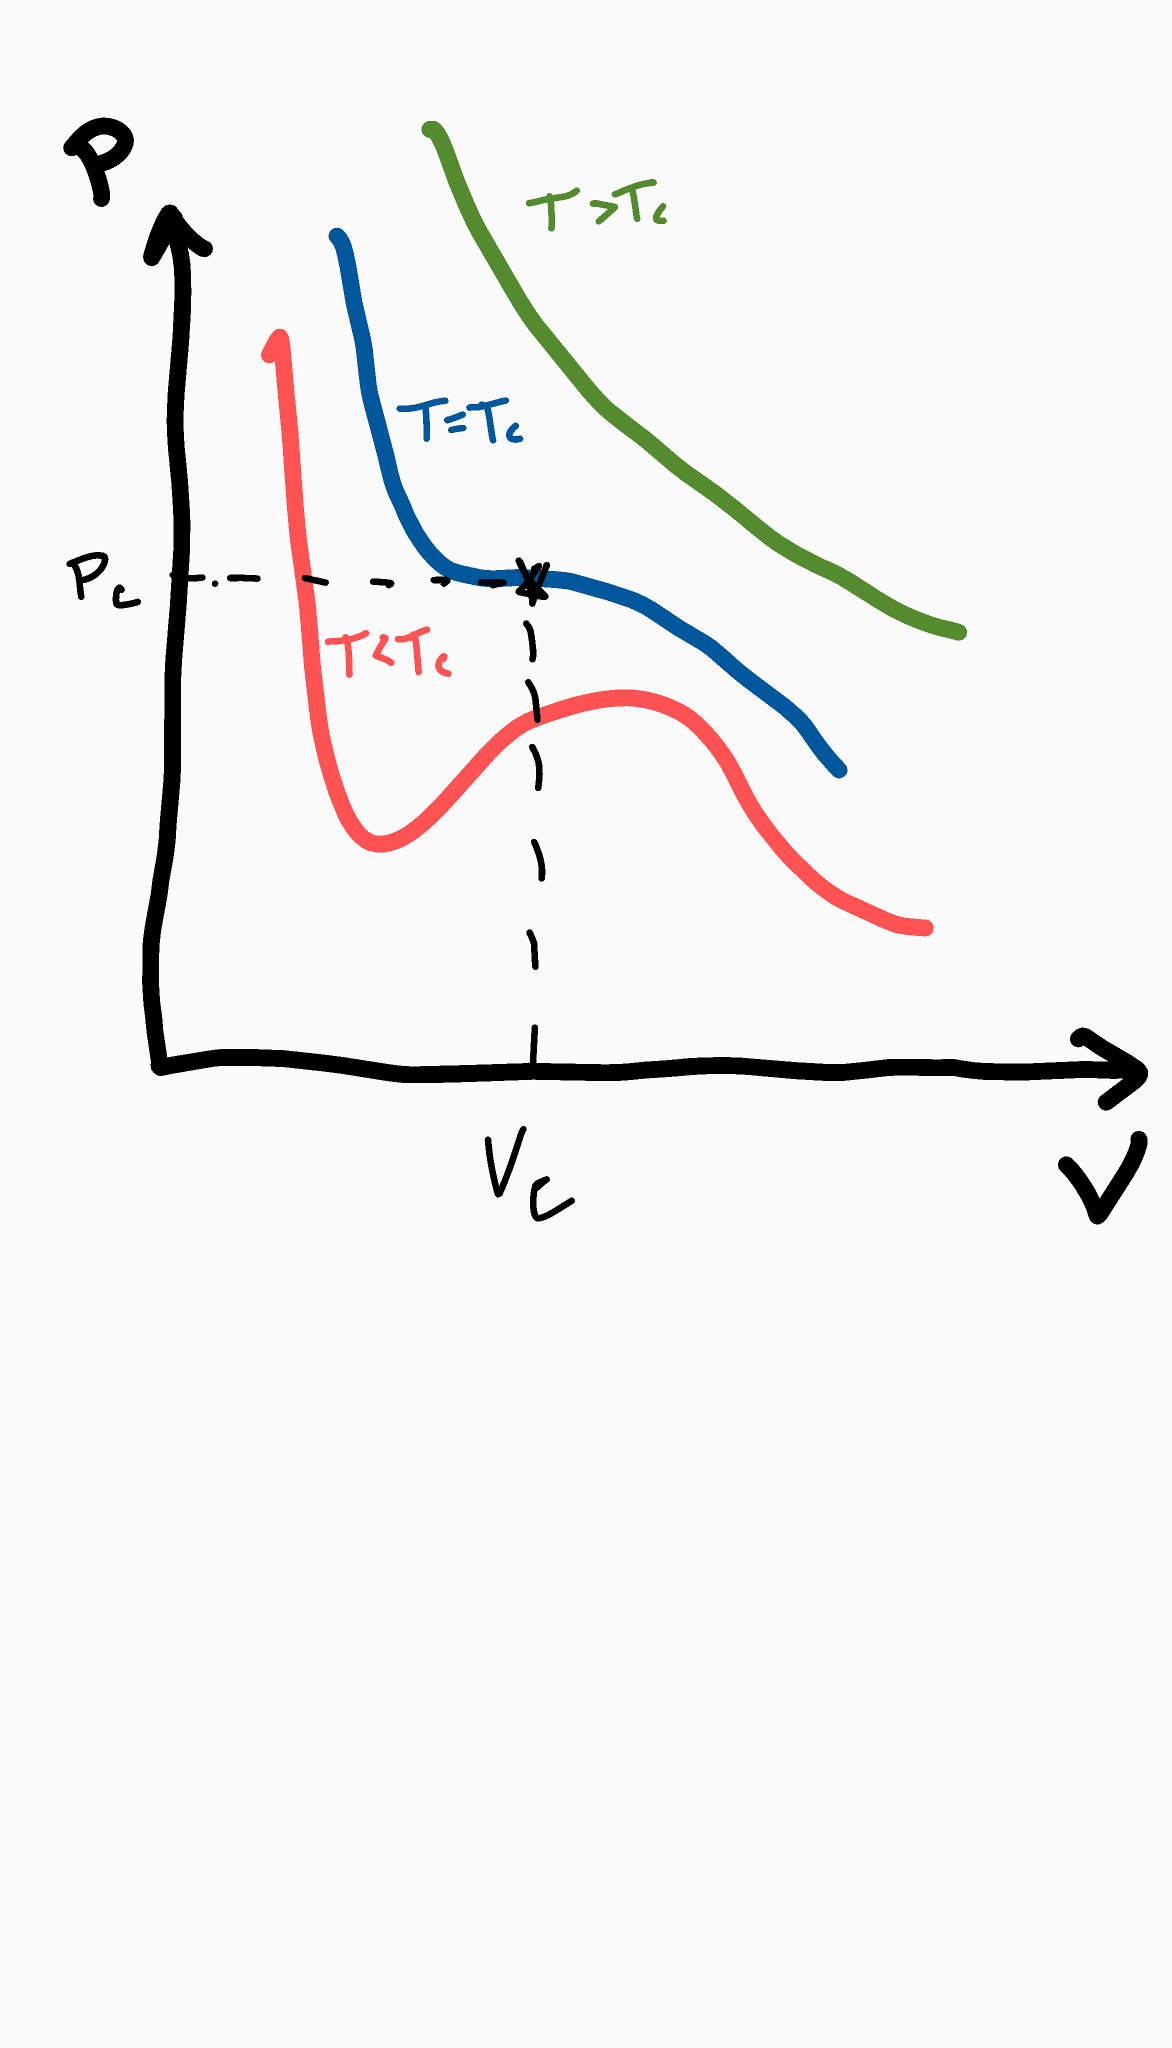
\includegraphics[width=3in]{Assignments/figa3.png}
}

\end{Solution}

\item Determine the temperature $T_{c}$ and the corresponding volume $V_{c}$ and pressure $p_{c}$

\begin{Solution}
The critical point occurs when $\left.\frac{\partial p}{\partial V}\right|_{T_{crit}} = 0$, $\left.\frac{\partial^2 p}{{\partial V}^2}\right|_{T_{crit}}$ and also $\left.\frac{\partial \mathcal{P}}{\partial \mathcal{V}}\right|_{T_{crit}} = 0$, $\left.\frac{\partial^2 \mathcal{P}}{{\partial \mathcal{V}}^2}\right|_{T_{crit}}$
\end{Solution}

\item Write the van der Waals equation in terms of state variables relative to the critical values, i.e. $\mathcal{T}=T / T_{c}$ and the corresponding volume $\mathcal{V}=V / V_{c}$ and pressure $\mathcal{P}=p / p_{c}$

\begin{Solution}
\begin{equation}
    \left.\frac{\partial p}{\partial V}\right|_{T_{crit}} = -\frac{RT}{\left(v-b\right)^2} + \frac{2a}{v^3} = 0
\end{equation}
\begin{equation}
    \left.\frac{\partial^2 p}{{\partial V}^2}\right|_{T_{crit}} = -\frac{2RT}{\left(v-b\right)^3} - \frac{6a}{v^4} = 0
\end{equation}
This leads to,
\begin{equation}
    a = \frac{9}{8}RT_{crit}v_{crit}, \qquad b = \frac{v_{crit}}{3}
\end{equation}
this lets us express the van der Waal equation as 
\begin{equation}
    \mathcal{V}^3-\frac{8}{3}\frac{\mathcal{T}\mathcal{V}^2}{\mathcal{P}} + \frac{\mathcal{V}^2}{3} + \frac{3\mathcal{V}}{P} - \frac{1}{\mathcal{P}} = 0
\end{equation}

\end{Solution}

    
\end{enumerate}

\newpage

%%%%%%%%%%%%%%%%%%%%%%%%%%%%%%%%%%%%%%%%%%%%%%%%%%%%%%%



\item \textbf{Barometric formula, isothermal atmosphere}

\begin{enumerate}

\item From the free energy of an ideal gas (which we derive later in this course),
$$
F=-N k T\left[\ln \left(\frac{n_{Q} V Z_{i n t}}{N}\right)+1\right]
$$
calculate the chemical potential.

\begin{Solution}
\begin{equation}
    \mu_{chem} = \frac{\partial F}{\partial N} = -k T\ln{\left(\frac{n_{Q} V Z_{i n t}}{N}\right)}
\end{equation}
\end{Solution}
\end{enumerate}
Now consider an ideal mono-atomic gas (atomic mass $M, Z_{\text {int}}=1$ ) in a uniform gravitational field and at constant temperature. Note: The solution will not depend on $n_{Q}$

\begin{enumerate}[resume]


\item What is the gravitational potential energy of an atom?

\begin{Solution}
\begin{equation}
    \mu_g = Mgh
\end{equation}
\end{Solution}

\item What is the chemical potential of this gas as a function of height $h$ and density $n=N / V ?$


\begin{Solution}
\begin{equation}
    \mu = k T \ln{\left(\frac{n}{n_Q}\right)} + Mgh
\end{equation}
\end{Solution}

\item Using the chemical potential, calculate the density as a function of height
$h$ and temperature $T .$ Assume $n(h=0)=n_{0}$


\begin{Solution}
\begin{equation}
\frac{n}{n_Q} = e^{\frac{\mu - M g h}{kT}}
\end{equation}
\begin{equation}
n(h, T) = n_0e^{\frac{- M g h}{kT}}
\end{equation}
\end{Solution}

\item What is the pressure as a function of height $h ?$ Assume $p(h=0)=p_{0}$
 

\begin{Solution}
\begin{equation}
    \frac{pV}{N}\ln{\frac{n}{n_Q}} = M g h - C
\end{equation}
\begin{equation}
    \frac{p}{n}\ln{\frac{n}{n_Q}} = M g h - C
\end{equation}
\begin{equation}
    p(h) = \frac{nMgh}{\ln{\frac{n}{n_Q}}}+p_0
\end{equation}
\end{Solution}

    
\end{enumerate}
\newpage

%%%%%%%%%%%%%%%%%%%%%%%%%%%%%%%%%%%%%%%%%%%%%%%%%%%%%%%

\item \textbf{Surface tension}
The interface between two phases is described by a thermodynamic variable called the surface tension $\mathcal{S}$. It is defined in terms of the work required to increase the surface area $A$ by an amount $d A$ through work $d W=\mathcal{S} d A$


\begin{enumerate}

\item Show that the pressure inside a spherical drop of water of radius $R$ is larger than the outside pressure by $2 \mathcal{S} / \mathcal{R}$ by calculating the work done against surface tension in an infinitesimal change in radius. What is air pressure inside a soap bubble of radius $R ?$

\begin{Solution}
In terms of radius,
\begin{equation}
    d W = 4\pi S d\left[r^2\right] =4\pi S 2r dr 
\end{equation}
The work needed can also be expressed as, 
\begin{equation}
    dW = (P_{in}-P_\infty ) (4\pi r^2 dr)
\end{equation}
equating these expressions gives us,
\begin{equation}
    4\pi S 2r dr = (P_{in}-P_{\infty} ) (4\pi r^2 dr)
\end{equation}
\begin{equation}
    \boxed{\Delta p = \frac{2S}{r}}
\end{equation}
\end{Solution}

\end{enumerate}

A water droplet condenses on a solid surface. There are 3 surface tensions involved, $\mathcal{S}_{a w}, \mathcal{S}_{w s},$ and $\mathcal{S}_{s a},$ where $a, w,$ and $s$ refer to air, water, and solid, respectively.
\begin{enumerate}[resume]


\item Calculate the angle of contact by i) energy minimization and ii) force equilibrium. Make use of the natural symmetries of the problem.
 

\begin{Solution}
total energy is the sum of all the work. The change in the total energy needs to be zero to have equilibrium. 
\begin{equation}
    0 = [SdA]_{aw} +[SdA]_{as} +[SdA]_{sw}
\end{equation}
the surface area for $sw$ and $as$ sum to the total solid surface area, which is constant. 
\end{Solution}

\item Find the condition for the appearance of a water film (complete wetting).


\begin{Solution}

\end{Solution}

\item Consider the competition of gravity, which dominates on a large scale, and surface tension on a water droplet. Estimate the maximum size of water drops on a non-wetting surface for which they are not much deformed from an ideal spherical shape.

\begin{Solution}

\end{Solution}

    
\end{enumerate}
\end{enumerate}
\end{document}
